%!TEX root = ../main.tex
\chapter{Opgaveformulering}
Kassesystemet i Katrines Kælder skal opdateres, da dankort terminalen og kasseapparatet ikke er koblet sammen. Derfor ønsker Katrines Kælders bestyrelse og bestyrere at digitalisere kassesystemet.
\newline\newline
Brugerne af systemet er frivillige bartender, som er studerende på Ingeniør Højskolen Aarhus Katrinebjerg, dog skal systemet være intuitivt og nemt at bruge selv i stressede situationer.
\newline\newline
Systemet skal indeholde en brugergrænseflade, som skal indeholde knapper tilsvarende dem på det gamle kasseapparat samt et display med køb, beløb mm. 
\newline\newline
Grundet forretningsregler indenfor branchen skal kasseopgørelserne for omsætningerne opbevares i baren mindst et år. Dette har givet anledning til meget papir og arbejde, og man ønsker derfor at ændre dette. Man ønsker i stedet for at kasseopgørelserne bliver gemt på en database enten lokalt på barens egen PC
eller en af IHA’s servere.
\newline\newline
Fokuspunkterne i projektet vil være følgende:
\begin{itemize}
\item Systemet er i stand til at kommunikere med dankortterminalen i forhold til at sende beløb til
dankortterminalen og modtage godkendt/afvist.
\item Brugerinterfacet indeholder de nødvendige knapper (tilsvarende det gamle kasseapparat)
\item Kasseopgørelserne skal gemmes på en database.
\newline
\end{itemize}
Yderlige krav og specifikationer af systemet udspecificeres i samarbejde med Katrines Kælders bestyrelse
og bestyrere.

\begin{figure}[h]
    \centering
    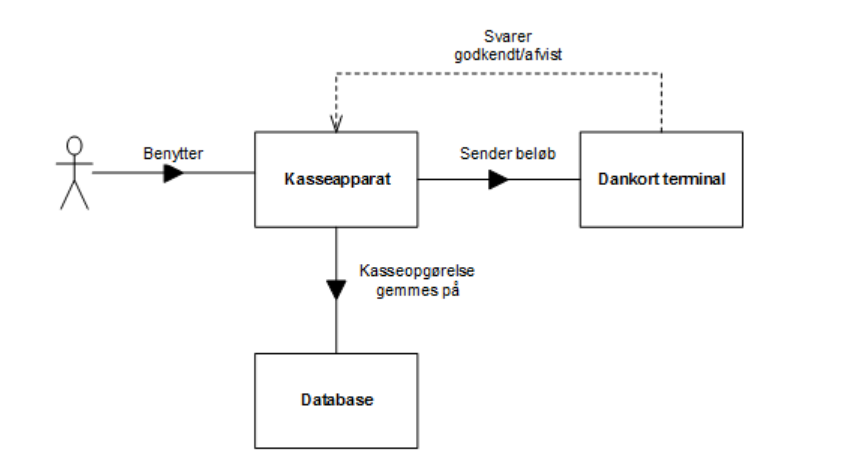
\includegraphics[width=0.8\textwidth]{Rapport/projektformulering.png}
    \caption{Kasseapparet}
    \label{fig:kasseapparat}
\end{figure}